\documentclass[12pt]{article}

%\usepackage{scicite}
\usepackage[sort&compress, numbers]{natbib}
\usepackage{times}
\usepackage{amssymb}
\usepackage{subfigure}
\usepackage{epsfig}
\usepackage{amsmath}
%\usepackage[colorlinks]{hyperref}
%\newcommand{\hah}[1]{\textcolor{magenta}{#1}}
%\newcommand{\tws}[1]{\textcolor{red}{#1}}

\topmargin 0.0cm
\oddsidemargin 0.2cm
\textwidth 16cm
\textheight 21cm
\footskip 1.0cm

\newenvironment{sciabstract}{%
\begin{quote} \bf}
{\end{quote}}

\title{Intramolecular Hole-Transfer in Protonated Anthracene}

\author
{Olha Krechkivska,$^{1}$ Callan M. Wilcox,$^{1}$ Klaas Nauta,$^{1}$ Scott H. Kable$^{1}$\\
and Timothy W. Schmidt$^{1,2\ast}$\\
\\
\normalsize{1. School of Chemistry, UNSW Sydney, NSW 2052, Australia}\\
\normalsize{2. ARC Centre of Excellence in Exciton Science, Australia}\\
\\
\normalsize{$^\ast$To whom correspondence should be addressed; E-mail:  timothy.schmidt@unsw.edu.au.}
}

\date{}

\begin{document}

\baselineskip24pt

\maketitle

\begin{abstract}
doo doo doo
\end{abstract}

\newpage
Charge transfer between two different molecules in an excited electronic state is at the heart of photosynthesis. This process is also mimicked in artificial devices which generate solar energy. In both organic photovoltaics (OPV) and dye-sensitized solar cells, following photon absorption, the excited state migrates and undergoes a charge transfer event. A detailed understanding of charge separation in OPV is hampered, in part, by the impossibility of detailed quantum chemical calculations on such a large system. In OPV devices, the electrons and holes are then conducted to metallic electrodes through a series of inter and intramolecular electron and hole-transfer processes.

Gas-phase laser spectroscopy offers the possibility to interrogate a well-defined, cold, isolated chemical system which is tractable at quantitative levels of electronic structure theory. To study photo-induced hole-transfer, a charged species must be studied, which engenders further experimental difficulties. Cations can be introduced into the gas phase by electrospray ionization, but the resulting species are not cold. Jet-cooled molecules can be ionized in the expansion region, but unless the ionization is at threshold, requiring tunable vacuum ultraviolet radiation, excess energy can be deposited in the cation. Techniques capable of studying jet-cooled, isomer-selected, cold cations are thus desirable.

The C$_{60}^+$ cation was recently studied by the photodissociation of its adduct with helium atoms in a 22-pole cryogenic ion trap. This technique affords a spectrum with a very small shift from the true gas phase spectrum. For C$_{60}^+$ cation this was sufficiently small to confirm the present of C$_{60}^+$ in interstellar space. Recently, we reported a triple-resonance technique whereby nascent cations were resonantly photodissociated following preparation by a resonant 2-colour 2-photon photon ionization process, at threshold. The result was an unambiguous spectrum of protonated naphthalene, isomer selected and vibrationally cold. Here we extend this treatment to protonated anthracene, which demonstrates symmetry-breaking in the excited state along a Marcus-Hush-like charge transfer coordinate.

Protonated anthracene has been studied previously. However, previous reports are neither at rigorously low vibrational temperature, nor isomer-selected. Garkusha et al. studied protonated anthracene in a cryogenic matrix, and Alata et al. created protonated anthracene (and other PAHs) in an electrical discharge containing H$_2$. The spectrum thus obtained contains many of the features of the present report, albeit at much lower resolution and higher temperature. In this study, we prepare 9-hydroanthracenium cations exclusively in their vibrational ground state by 2-color resonant ionization of the corresponding 9-dihydroanthracenyl radical. We show that the $C_{2v}$ ground state undergoes symmetry breaking in the excited state along a $b_2$ (in-plane) mode, effectively localizing the positive charge on one end of the molecule. This coordinate thus represents the abscissa of a Marcus diagram, and the excitation spectrum is interpreted from this standpoint.

\begin{figure}
\centering
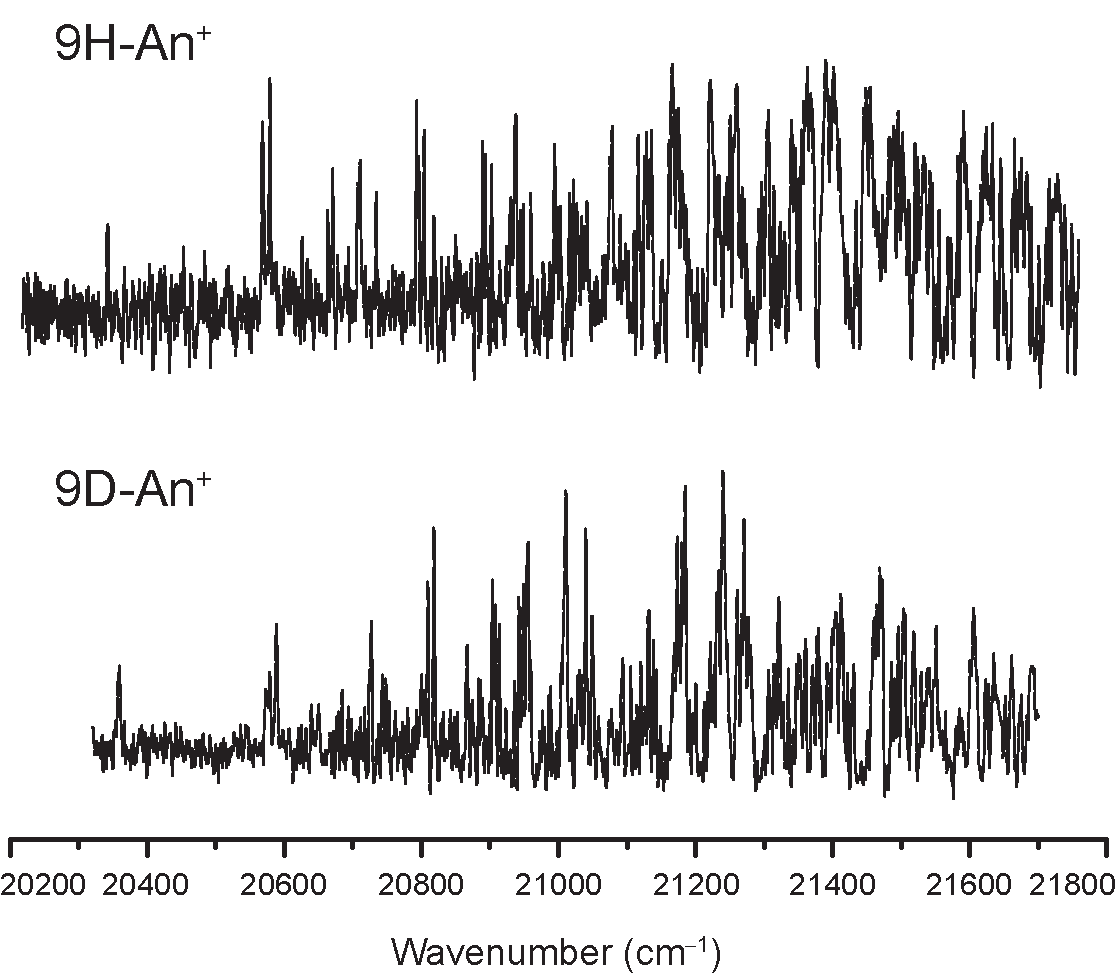
\includegraphics[width=12cm]{spectra}
\caption{Resonant photodissociation spectra of protonated and deuteronated anthracene. The cation was prepared by resonantly ionizing the 9H(D)-An neutral at threshold, guaranteeing cold, isomerically selected cations.\label{spectra}}
\end{figure}

\section*{Results}
The resonant photodissociation spectra of protonated and deuteronated anthracene are shown in Figure \ref{spectra}. The cations were prepared by resonantly ionizing the neutrals at threshold, and as such we can be certain that the spectra correspond to protonation (deuteronation) at the 9-position, the $C_{2v}$ species. The spectra reveal a number of progressions, possibly indicating a large geometry change between the ground and excited states of the cation.


\section*{Theoretical Considerations}
Anthracene protonated at the 9-position is considered $C_{2v}$ until proven otherwise. If the sp$^3$ carbon is considered as an insulator, the chromophore will consist of two aromatic rings linked by an sp$^2$-hybridized bridging carbon. The frontier orbitals of the aromatic rings can be taken in even and off combinations, resulting in sets of $b_1$ and $a_2$ symmetry. Only the $b_1$ set can interact with the bridge, which is also $b_1$. Of the highest occupied aromatic $b_1$ orbitals, one will have a node at the tertiary carbon atom adjacent to the bridge, and is not expected to be strongly perturbed. The other mixes with the bridging p-orbital and is lowered in energy. This results in two relatively unperturbed aromatic, symmetry-adapted orbitals of $a_2$ and $b_1$ symmetry. The lowest-energy unoccupied orbital is largely located on the bridge. The frontier orbitals are shown in Figure \ref{FIG1}.

The HOMO-LUMO transition of the cation is thus electron transfer from the aromatic rings to the bridge, corresponding to hole-transfer from the bridge onto the aromatic rings. This brings about two near-degenerate transitions to states of $A_1$ and $B_2$ symmetry. Distortion along a $b_2$ mode will reduce the point group to $C_s$ and render both these excited states $A'$. The interaction between these two states could potentially push the lower state to an energy below that of the $C_{2v}$ geometry.

The ground state geometry was calculated under $C_{2v}$ symmetry at the B3LYP/6-311+G(d,p) level of theory. All frequencies were found to be real, indicating a true minimum energy. The vertical excitation energy was calculated at the [10,11] MCQDPT2/6-311G(d,p) level of theory. The results are reported in Table \ref{tab1}.

The excited state optimized geometry was calculated at the TD-B3LYP/6-311+G(d,p) level of theory. All frequencies were found to be real. At this geometry, the lowest electronic states were calculaed at the [10,11] MCQDPT2/6-311G(d,p) level of theory with the results reported in Table \ref{tab1}.




\begin{table}
  \caption{Electronic State Energies$^a$ ($f$-values) Calculated at the [10,11] MCQDPT2/6-311G(d,p) and TD-B3LYP/6-311+G(d,p) Levels of Theory\label{tab1}}
  \centering
  \begin{tabular}{lrrrr}
    \hline\hline
      & \multicolumn{2}{c}{$C_{2v}$} &  \multicolumn{2}{c}{$C_s$}\\
      \cline{2-5}
      & MCQDPT2 & TD-B3LYP & MCQDPT2 & (TD)-B3LYP\\
      \hline
State \\
$1^1A_1$ & 0            & 0     & 2634  &  1249\\
$2^1A_1$ & 22081 (0.04) & 19376 (0.02) & 20928 (0.03) & 18939 (0.01)\\
$1^1B_2$ & 24350 (0.29) & 22384 (0.00) & 25989 (0.02) & 25147 (0.01)\\
$2^1B_2$ & 25088 (0.39) & 26819 (0.50) & 27492 (0.59) & 27819 (0.48)\\
 \end{tabular}
 
 $a$ cm$^{-1}$
\end{table}





C2v A1 0.794276 E*BOHR
Cs     0.676497 E*BOHR

 Excited State   1:      Singlet-A1     2.4023 eV  516.10 nm  f=0.0175  <S**2>=0.000
      47 -> 48         0.70530
 This state for optimization and/or second-order correction.
 Total Energy, E(TD-HF/TD-DFT) =  -539.915220713
 Copying the excited state density for this state as the 1-particle RhoCI density.

 Excited State   2:      Singlet-B2     2.7753 eV  446.74 nm  f=0.0011  <S**2>=0.000
      45 -> 48        -0.32715
      46 -> 48         0.62477

 Excited State   3:      Singlet-B2     3.3251 eV  372.87 nm  f=0.5030  <S**2>=0.000
      45 -> 48         0.62125
      46 -> 48         0.32818

 Excited State   4:      Singlet-A1     4.6104 eV  268.92 nm  f=0.0204  <S**2>=0.000
      44 -> 48         0.66485
      45 -> 50        -0.12853
      47 -> 49         0.16064



 Excited State   1:      Singlet-A'     2.1933 eV  565.28 nm  f=0.0096  <S**2>=0.000
      47 -> 48         0.70452
 This state for optimization and/or second-order correction.
 Total Energy, E(TD-HF/TD-DFT) =  -539.917209976
 Copying the excited state density for this state as the 1-particle RhoCI density.

 Excited State   2:      Singlet-A'     2.9629 eV  418.45 nm  f=0.0090  <S**2>=0.000
      45 -> 48         0.68272
      46 -> 48        -0.16940

 Excited State   3:      Singlet-A'     3.2943 eV  376.36 nm  f=0.4814  <S**2>=0.000
      45 -> 48         0.16580
      46 -> 48         0.68156

 Excited State   4:      Singlet-A"     4.5067 eV  275.11 nm  f=0.0001  <S**2>=0.000
      43 -> 48         0.70202

-539.9978138

\section*{Conclusions}



\section*{Methods}


\section*{Data Availability}

\section*{Acknowledgements}


%\section*{Author Contributions}
%....

%\section*{Competing Financial Interests}
%There are no competing financial interests.

%\bibliography{scibib}
%\bibliographystyle{naturemag}

%\section*{Supplementary Information}
%Detailed Materials and Methods\\
%Supplementary Figures X to X\\
%Supplementary Table X

%\newpage

%\section*{Figure Legends}
%Figure 1:

%\newpage
% put all the figures here later on with a \newpage in between.



\end{document}


